% !TeX spellcheck = en_US
\documentclass[a4paper,14pt]{extarticle}
\usepackage[left=2.5cm, right=1.5cm, vmargin=2.5cm]{geometry}
\usepackage[utf8]{inputenc}
\usepackage[T2A]{fontenc}
\usepackage[russian]{babel}
\usepackage{graphicx}
\graphicspath{{pictures/}}
\usepackage{caption}
\usepackage{subcaption}
\usepackage{indentfirst}
\setlength\parindent{5ex}
\usepackage{fancyhdr}
\usepackage{booktabs}
\usepackage{siunitx} 
\usepackage{pgfplotstable}
\usepackage{amsmath}
\usepackage{autonum}
\usepackage{amsfonts}
\DeclareMathOperator{\sign}{sgn}
\newcommand{\gt}{\textgreater} % знак больше
\newcommand{\lt}{\textless}       % знак меньше
\DeclareGraphicsExtensions{.pdf,.png,.jpg}
\pagestyle{fancy}
\fancyhf{}
\rhead{\thepage}
\renewcommand{\headrulewidth}{0pt}

\fancypagestyle{plain}{ 
	\fancyhf{}
	\rhead{\thepage}}

\author{Никитин Илья}

\title{Отчет по лабораторной работе №3: "Длинные линии"}
\date{\today}

\begin{document}
	
	\maketitle
	\tableofcontents

	\section{Оборудование}
	
	\section{Задачи}
	
	\section{Теория}
		Длинной линией называют электрическую цепь, образованную двумя параллельно идущими проводниками, длина которых сравнима или больше длины волны передаваемого сигнала.
		\subsection{Телеграфные уравнения}
			Длинную линию можно разбить на короткие отрезки длиной много меньшей длины волны передаваемого сигнала. Такой отрезок обладает погонными сопротивлением $R$, проводимостью $G$, емкостью $C$ и индуктивностью $L$. Распределение тока и напряжения вдоль линии описываются системой телеграфных уравнений:
			\begin{equation}
				\begin{cases}
					\frac{\partial U}{\partial x} = -L \frac{\partial J}{\partial t} - R J;\\						\frac{\partial J}{\partial x} = -C \frac{\partial U}{\partial t} - G U.
				\end{cases}
			\end{equation}
		 	В идеальной линии без потерь эти уравнения сводятся к волновому уравнению для напряжения:
		 	\begin{equation}
				\frac{\partial^2 U}{\partial x^2} -\frac{1}{U^2} \frac{\partial^2 U}{\partial t^2} = 0.
		 	\end{equation}
		 	Скорость распространения волн: $u = \frac{1}{\sqrt{L C}}$
		 \subsection{Гармонические волны в линии}
		 	Поскольку телеграфные уравнения линейны по току и напряжению, то можно свести вопрос о распространении сигнала произвольной формы к вопросу о распространении гармонического сигнала. Если в точке $x = 0$ линии включен источник переменного напряжения $U(t) = U_0 \exp{i \omega t}$, то в линии с потерями будет две волны: распространяющаяся от источника и отраженная от второго конца линии:
		 	\begin{equation}
		 		U(x,t) = U_0 \exp{(i \omega t)} (A \cdot \exp{(-\gamma x)} + B \cdot \exp{(\gamma x)}),
		 	\end{equation}
		 	где $\gamma = \sqrt{(R + i \omega L)(G + i \omega C)}$ - комплексная постоянная распространения. Величина $\alpha = Re{\gamma}$ называется коэффициентом затухания а $\beta = Im{\omega}$ носит название фазовой постоянной. Длиной волны называется величина $\lambda = \frac{2 \Pi}{\beta}$
		 	\newline
		 	Если отраженной волны нет, то ток и напряжение в любом сечении линии связаны соотношением:
		 	\begin{equation}
		 		\frac{U}{J} = \Omega \equiv \sqrt{\frac{R+ i \omega L}{G + i \omega C}}
		 	\end{equation}
		 	Величина $\Omega$ называется волновым сопротивлением линии.
		 	
		 	На практике часто реализуется случай малых потерь, когда $R \ll \omega L$ и $G \ll \omega C$. Кроме того почти всегда потерями через проводимость можно пренебречь. В таком случае $\Omega \approx \sqrt{L / C}$ и
		 	\begin{equation}
		 		\alpha \approx \frac{R}{2 \Omega}; \quad \beta \approx \omega \sqrt{L C}.
		 	\end{equation}
		 \subsection{Коэффициент отражения и прохождения.}
		 	Пусть $r_u(x)$ - это отношение амплитуд падающей и отраженной волн, вычисленное в точке x. В линии с волновым сопротивлением $\Omega$, нагруженной на импеданс $Z$, коэффициент отражения непосредственно вблизи нагрузки (т.е. при $x = l$):
		 	\begin{equation}
		 		r_u(l) = \frac{A \exp{(-\gamma l)}}{B \exp{(\gamma l)}} = \frac{Z - \Omega}{Z + \Omega}
		 	\end{equation}
		 	При разомкнутой линии $r_u = 1$, в замкнутой $r_u = -1 $, а при $Z = \Omega$ отраженной волны не возникает вовсе: $r_u = 0$.

		 	Коэффициентом прохождения называют отношение комплексных амплитуд падающей волны на входе и выходе из линии:
		 	\begin{equation}
		 		S_{1 2} = \exp(-\gamma l) \frac{1 + r_u}{1 + r_u \exp{(-2 \gamma l)}}.
		 	\end{equation}
		 	Если на выход подключена согласованная нагрузка, то $r_u = 0$ и $S_{1 2} = \exp{(-\gamma l)}$
		 \subsection{Входное сопротивление}
		 Входным сопротивлением длинной линии называют отношение напряжения к току на входе в линию: $Z_{in} = \left. (U/J)\right|_{x = 0}$. Входное сопротивление линии, нагруженной на импеднс $Z$, равно
		 \begin{equation}
		 	Z_{in} = Z \frac{1 + \frac{\Omega}{Z} \tanh(\gamma l)}{1 + \frac{Z}{\Omega} \tanh(\gamma l)}
		 \end{equation}
		 Если второй конец линии замкнут, то $Z_{in} = \Omega \coth(\gamma l)$; для разомкнутого конца $Z_{in} = \Omega \tanh(\gamma l)$, а для согласованной линии $Z_{in} = \Omega$. При тех значениях частоты, при которых на длине линии укладывается число волн, кратное $1/4$, поведение длинной линии напоминает поведение последовательного или параллельного колебательного контура. В максимумах значение модуля сопротивления
		 \begin{equation}
		 	Z_{max} \approx \Omega^2 /(2 R l), 
		 \end{equation}
	\subsection{Способы согласования}
		Зачастую возникает необходимость в том, чтобы при нагружении линии на заданный резистор $R_{load}$ не возникало отраженных сигналов. Для этого использются различные методы согласования линии и нагрузки. Если сопротивление нагрузки $R_{load}$ больше волнового сопротивления линии $\Omega$, то можно подключить резистор сопротивлением $r = R_{load} - \Omega$. Если же сопротивление нагрузки меньше волнового сопротивления, то можно параллельно нагрузке подключить резистор $r = R_{load} \cdot \Omega / (R_{load} - \Omega)$.
	\subsection{Погонные параметры}
		Пусть $а$ - внешний диаметр жилы, $b$ - внутренний диаметр оплетки, $\epsilon$ и $\mu$ - диэлектрическая и магнитная проницаемости диэлектрика, $\rho_{1,2}$ - удельное сопротивление материалов жилы и оплетки по постоянному току. Тогда погонная емкость коаксиального кабеля задается формулой
		\begin{equation}
			C = \frac{2 \pi \epsilon_0 \epsilon}{\ln(b / a)} \approx \frac{56 \epsilon}{\ln(b / a)} \quad [\text{пФ/м}].
		\end{equation}
		Погонная индуктивность и сопротивление уже зависят от частоты $f = \omega / (2 \pi)$ из-за скин-эффекта: высокочастотные токи выталкиваются из объема проводника и концентрируются в тонком слое толщиной
		\begin{equation}
			\delta = \sqrt{\frac{\rho}{\pi \mu_0 f}}
		\end{equation}
		Формула для индуктивности на высоких (выше 100 кГц) частотах:
		\begin{equation}
			L = \frac{\mu_0 \mu}{4 \pi} \ln(b / a) + \frac{\sqrt{\mu_0}}{6 \pi^{3/2}} (\frac{k_1 \sqrt{\rho_1}}{a} + \frac{k_2 \sqrt{\rho_2}}{b}) \frac{1}{\sqrt{f}}
		\end{equation}
		где $k_1, k_2$ - безразмерные коэффициенты порядка единицы, зависящие от конструктивных особенностей кабеля. Для кабеля с жилой, состоящей из одного провода и сплошным экраном $k_1 = k_2 = 1$. Вклад от второго слагаемого мал по сравнению со вкладом от первого, поэтому обычно пользуются приближенной формулой
		\begin{equation}
			L \equiv L_{\infty} = \frac{\mu_0 \mu}{4 \pi} \ln{b / a} \approx 0.2 \mu \ln{b / a} \quad[\text{мкГн/м}]
		\end{equation}
		Сопротивление возрастает с ростом частоты по корневому закону:
		\begin{equation}
			R = \frac{k_1 \rho_1}{2 \pi a \delta_1} + \frac{k_2 \rho_2}{2 \pi a \delta_2} = \frac{1}{2} \sqrt{\frac{\mu_0}{\pi}} (\frac{k_1 \sqrt{\rho_1}}{a} + \frac{k_2 \sqrt{\rho_2}}{b}) \sqrt{f}.
		\end{equation}
		Подставляя выражения для индуктивности и емкости в формулы скорости распространения волн и волнового сопротивления, находим:
		\begin{equation}
			u = \frac{c}{\sqrt{\epsilon \mu}}, \quad \Omega = \frac{1}{2 \pi} \sqrt{\frac{\mu_0 \mu}{\epsilon_0 \epsilon}} \ln{b / a} \approx 60 \sqrt{\frac{\mu}{\epsilon}} \ln{b / a} \quad[\text{Ом}].
		\end{equation}
	\section{Геометрические размеры и волновое сопротивление}
		\subsection{Ход работы}
		В первую очередь мы измерили и записали геометрические параметры кабеля. Радиус внешней оболочки и внутреннего провода получились следующими:
		\begin{equation}
			\begin{gathered}
				R = 1.534 \pm 0.001 \; \text{мм} \\
				r = 0.200 \pm 0.001 \; \text{мм}
			\end{gathered}
		\end{equation}
		Для измерения волнового сопротивления $\Omega$ мы воспользовались схемой, приведенной на рисунке. Сигнал с генератора осциллографа подается на тройник, присоединяющийся одной стороной ко входу осциллографа. К оставшейся стороне тройника присоединяется исследуемый коаксиальный кабель. Сначала свободный конец кабеля остается разомкнутым.
		\begin{figure}[h!]
			\centering
			\includegraphics[width=.75\linewidth]{схема.png}
			\caption{Схема для определения волнового сопротивления}
			\label{fig1}
		\end{figure}
		На генераторе устанавливается прямоугольный сигнал (меандр), который отражается от свободного конца кабеля. Подобрав должным образом период и длительность сигнала можно добиться того, что на экране осциллографа будет видо два прямоугольных импулься в течение одного периода: поступающий с генератора отраженный от второго конца кабеля. Их довольно легко различить, так как из-за затухания и дисперсии в кабеле амплитуда отраженного импульса меньше, а его форму немного меняется.
		
		Если теперь нагрузить свободный конец кабеля на переменный резистор $R_x$, то амплитуда отраженного сигнала изменится. Подбирая различные значения $R_x$ сопротивления переменного резистора, можно добиться отсутствия отраженного сигнала. Это произойдет при значении $R_x$, равном $\Omega$.
		
		Получившееся значение волнового сопротивления:
		\begin{equation}
			\Omega = 53.72 \pm 0.01 \; \text{Ом}
		\end{equation}
	\section{Скорость распространения волн}
		\subsection{Ход работы}
			Используя ту же схему, что и в предыдущем опыте, но с разомкнутым свободным концом, можно, изменяя период и длительность прямоугольного сигнала, добиться такой ситуации, при которой сигнал с генератора начинает перекрываться с отраженным сигналом. Можно проверить, что длительность $\tau$ двух "ступенек" слева и справа от центральной ступеньки не зависит ни от периода прямоугольного сигнала, ни от длительности (покуда только сигнал с генератора и отраженный сигнал перекрываются), и равна $l / u$.
			
			Получившееся значение волнового сопротивления:
			\begin{equation}
				u = 1.2 \cdot 10^8 \frac{\text{м}}{\text{с}}
			\end{equation}
	\section{Входное сопротивление длинной линии}
		\subsection{Ход работы}
			Для измерения входного сопротивления использовалась схема, приведенная на рисунке. Измеряя при помощи осциллографа напряжения $U_1$ и $U_2$ по разные стороны от резистора R, мы можем рассчитать силу тока $J$, а деля $U_2$ на $J$ получим, по определению, входной импеданс длинной линии $Z_{in}(f)= \frac{U_2}{J}$. Использовался резистор сопротивлением $R = 195 \; \text{Ом}$.
			\begin{figure}[h!]
				\centering
				\includegraphics[width=.85\linewidth]{схема2.png}
				\caption{Схема для определения входного сопротивления}
				\label{fig2}
			\end{figure}
			\newpage
			С помощью схемы были измерены входные сопротивления разомкнутой, замкнутой накоротко и нагруженной на согласованную нагрузку длинной линии.
		\subsection{Обработка данных}
			С помощью программы на LabView и дальнейшей обработки был получен график зависимости модуля входного сопротивления от частоты.
			\begin{figure}[h!]
				\centering
				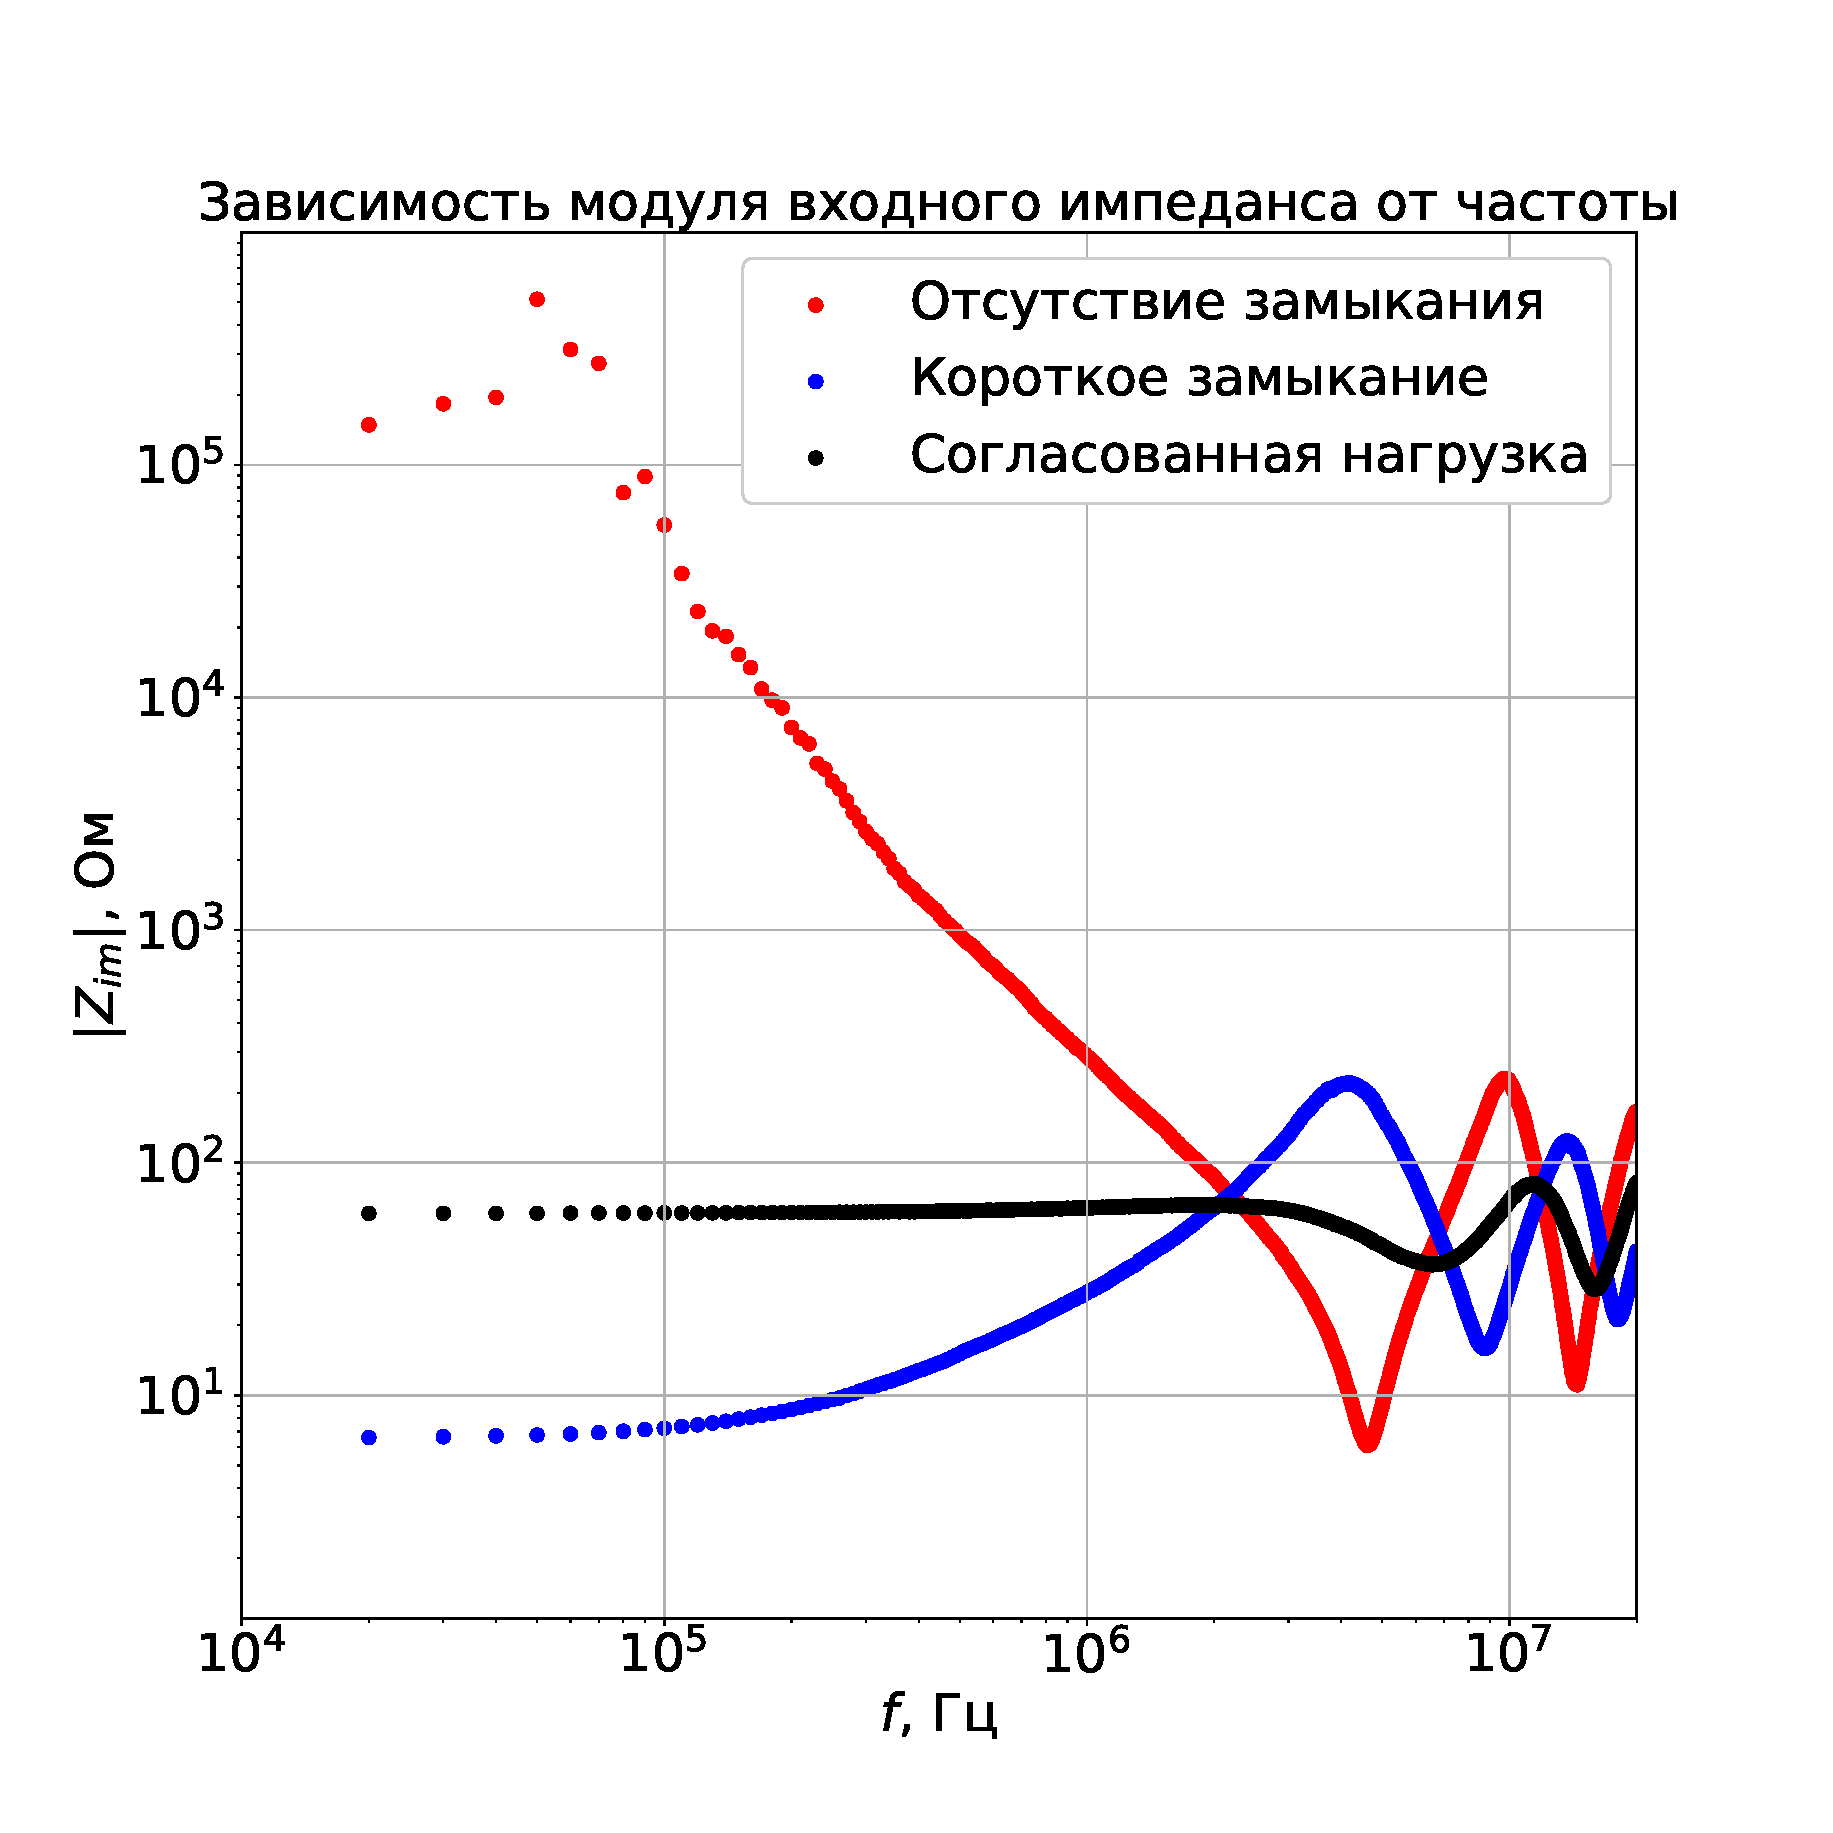
\includegraphics[width=.75\linewidth]{Lab3_1.eps}
				\caption{Зависимость модуля входного импеданса от частоты}
				\label{fig3}
			\end{figure}
			\newpage
			Графики для удобства нарисованы в логарифмических координатах. Нас интересуют значения максимумов модуля входного импеданса от частоты на разомкнутой и замкнутой накоротко схемах, с помощью которых мы расчитаем значения удельного сопротивления кабеля. Беря в расчет только максимумы графика короткого замыкания (остальные значения резко выпадают), получим:
			\begin{equation}
				\rho \approx 3.3 \cdot 10^{-8} \; \text{Ом}\cdot\text{м}
			\end{equation}
	\section{Коэффициент прохождения}
		\subsection{Ход работы}
		Для измерения коэффициента прохождения $S_{1 2}(f)$ используется векторный анализатор цепей. Исследуемый кабель подключается к двум входам анализатора цепей, который "запускает" гармонический сигнал из входа 1 в кабель и регистрирует сигнал, пришедший на второй вход.
		
		Оба входа анализатора цепей имеют сопротивление $50 \; \text{Ом}$, поэтому для кабеля, у которого волновое сопротивление совпадает с этим значением, коэффициент прохождения задается просто выражением $S_{1 2} = \exp(-\gamma l)$. Если сопротивление отличается, то можно применить общую формулу.
		
		Исследуя зависимость амплитуды и фазы коэффициента прохождения от частоты и считая потери малыми (т.е. $\alpha l \ll 1$), мы можем, воспользовавшись формулами найти, как зависят погонные индуктивность и сопротивление от частоты. Также можно оценить сопротивление материала жилы и оплетки.
		\subsection{Обработка данных}
		Сначала я построил график зависимости коэффициента затухания и фазовой постоянной от частоты
		\begin{figure}[h!]
			\centering
			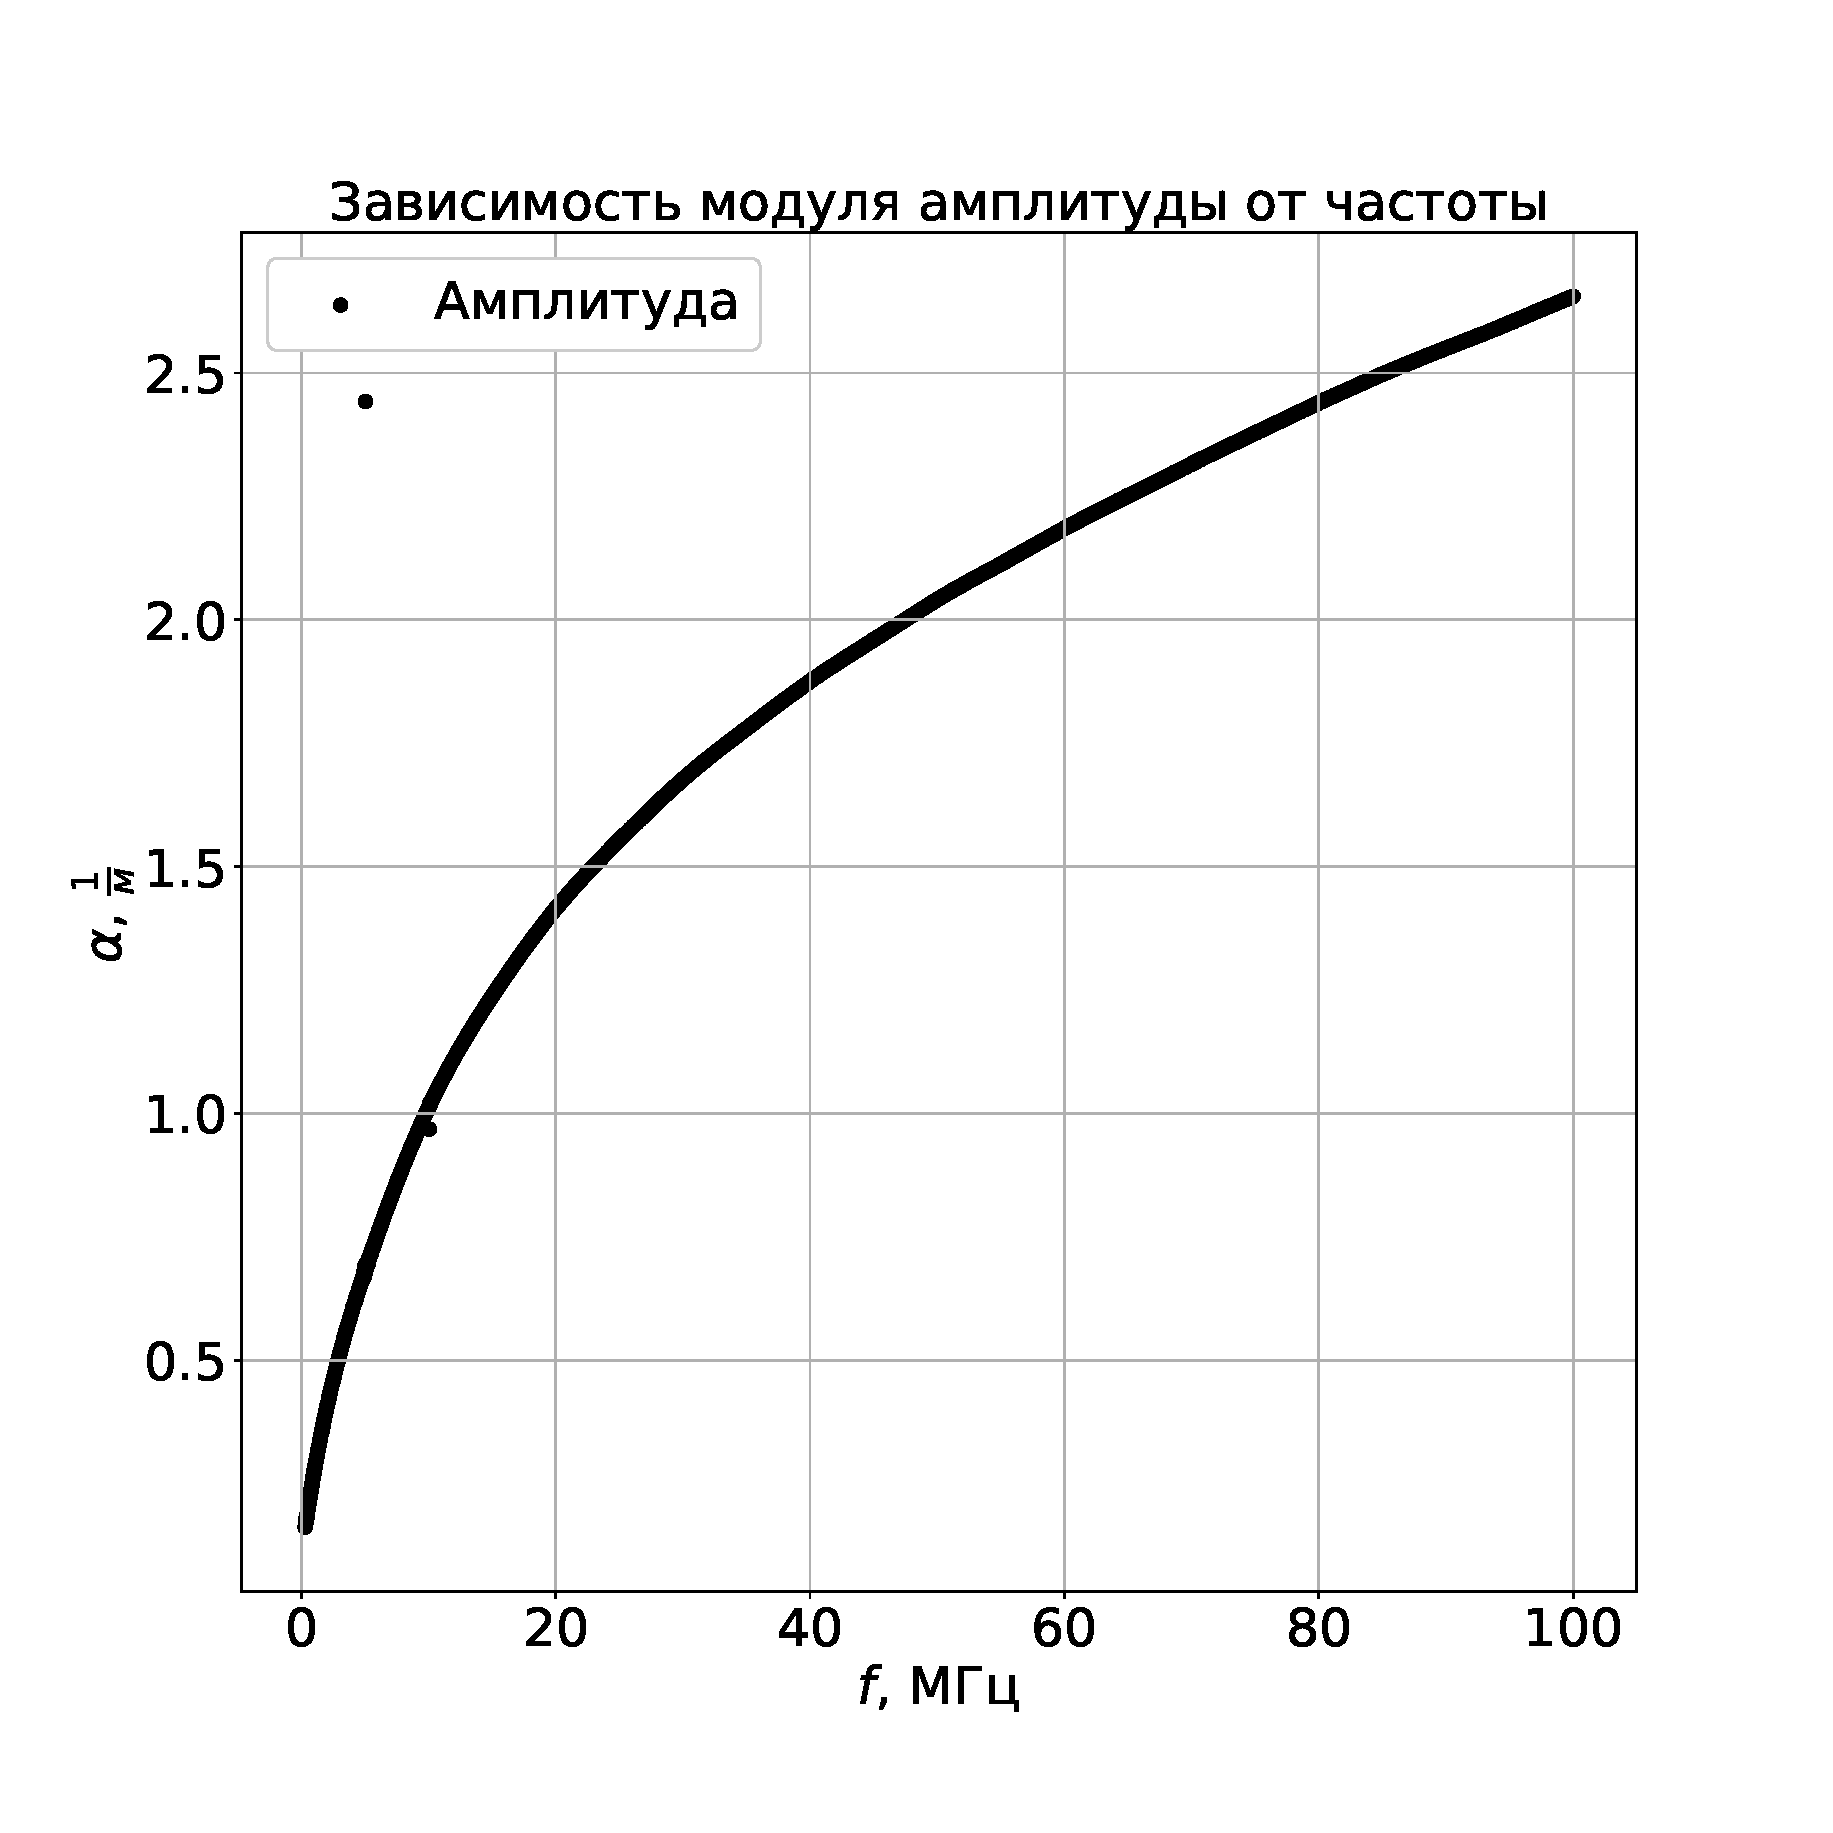
\includegraphics[width=.75\linewidth]{Lab3_2.eps}
			\caption{Зависимость модуля коэффициента затухания от частоты}
			\label{fig4}
		\end{figure}
		\newpage
		\begin{figure}[h!]
			\centering
			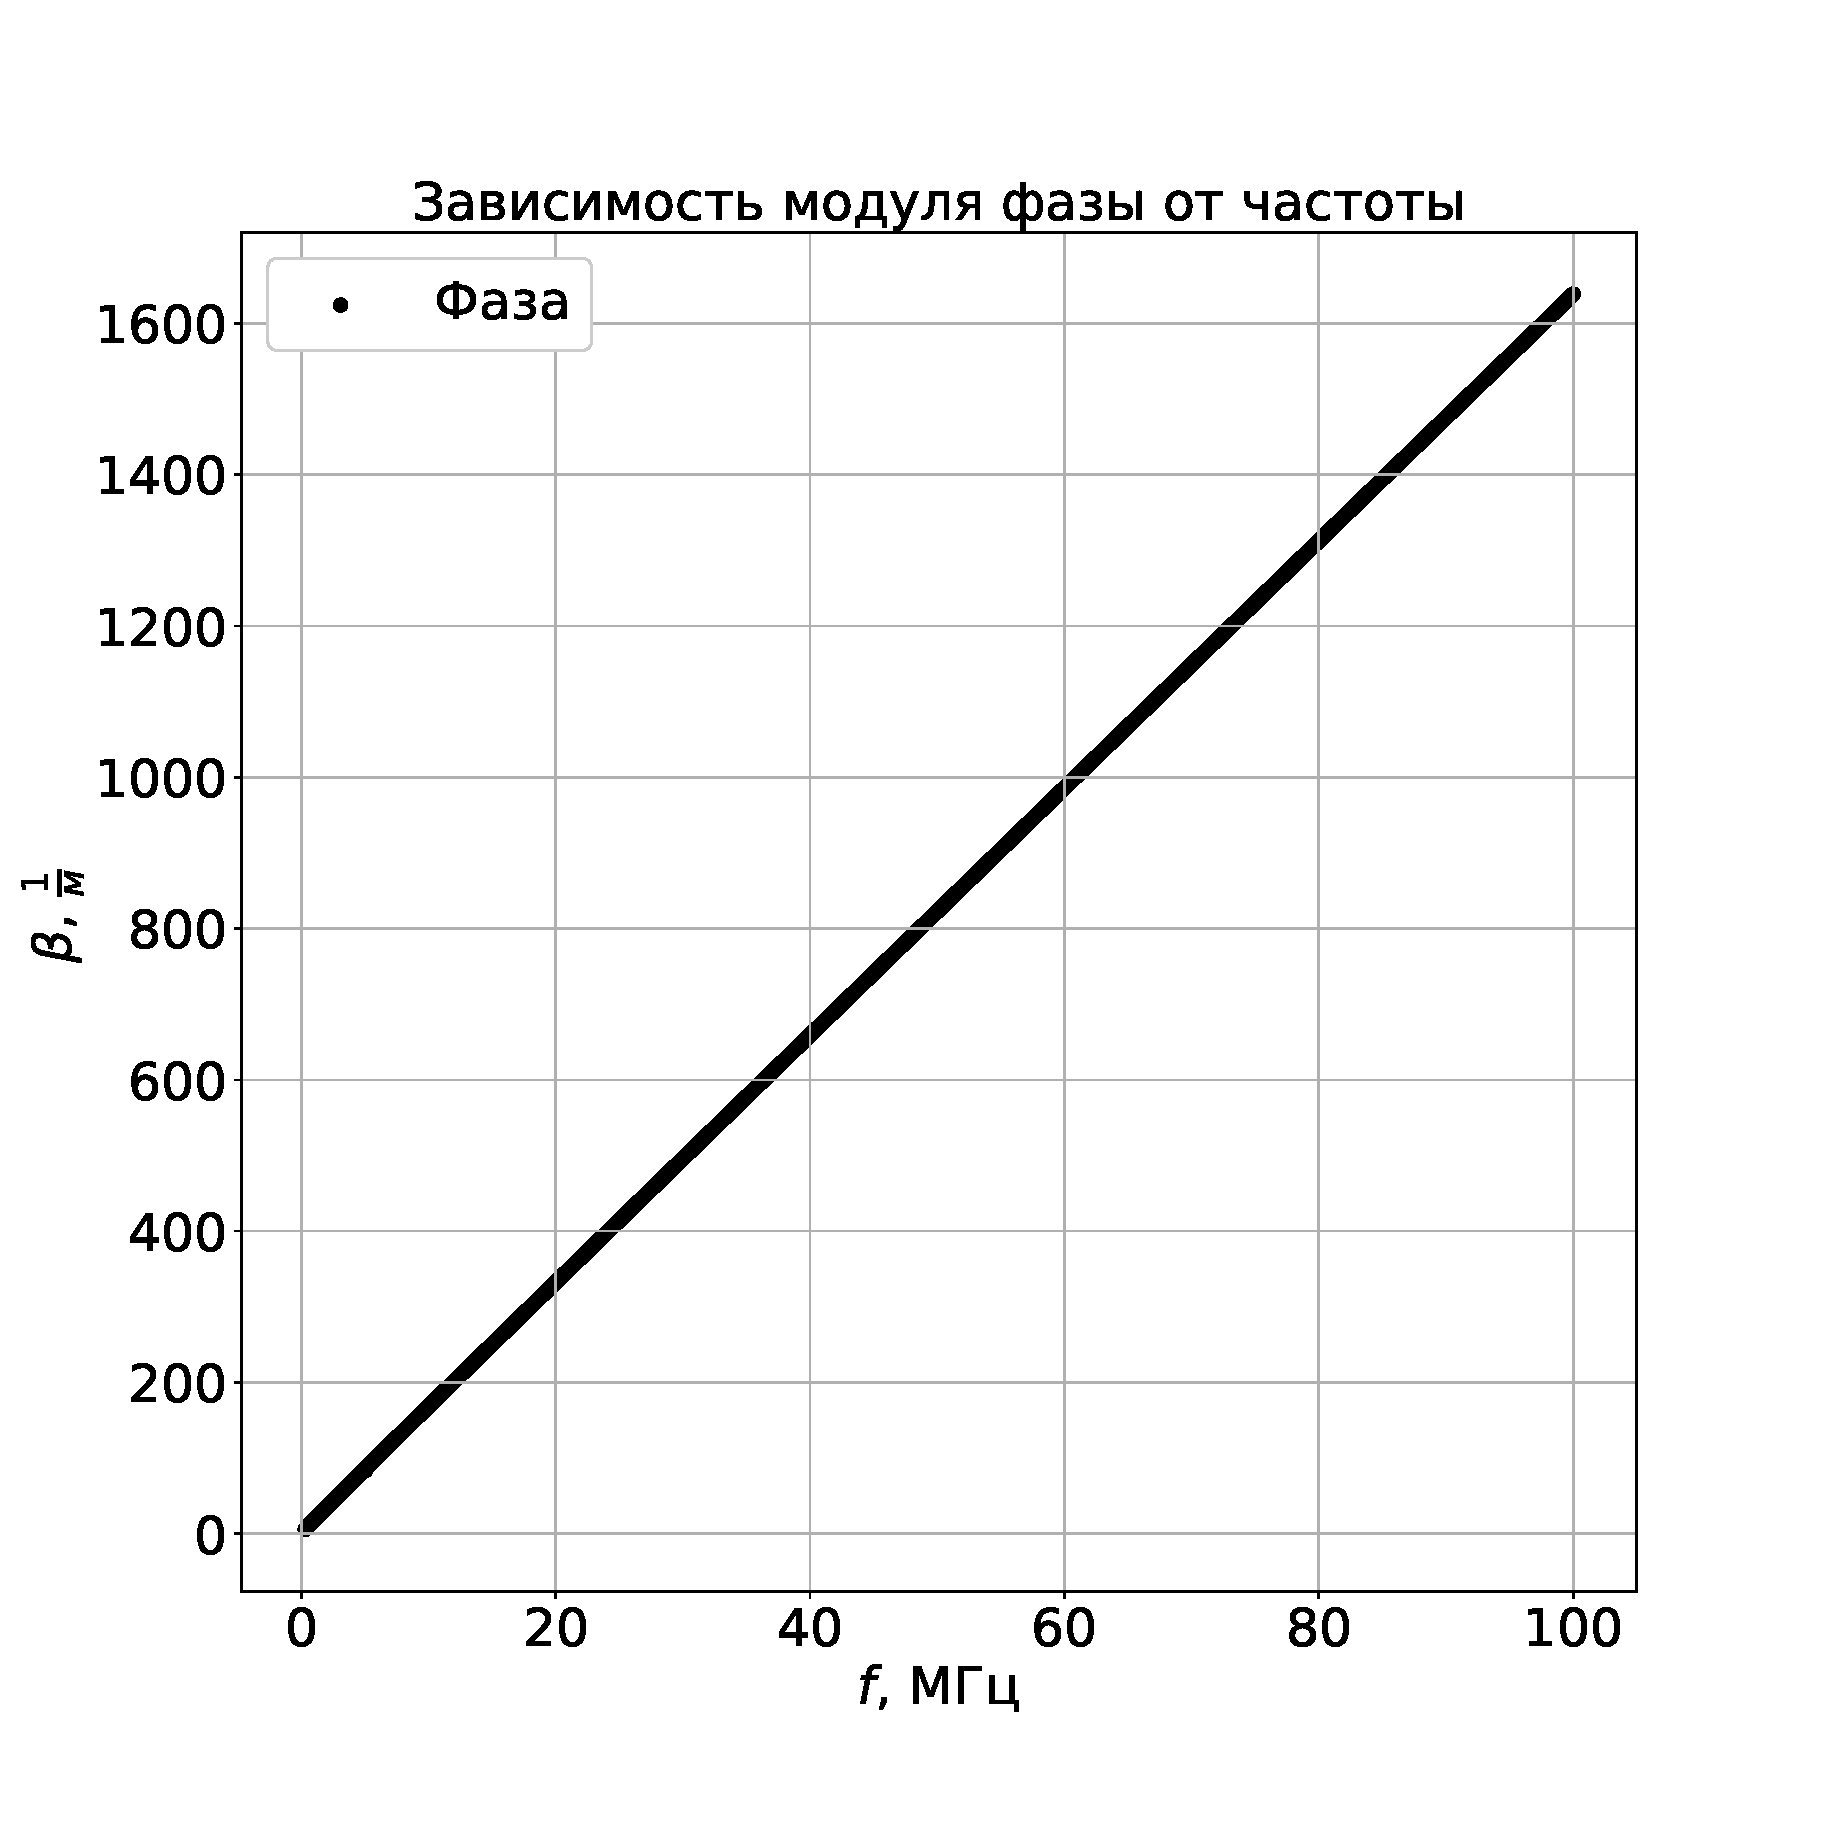
\includegraphics[width=.75\linewidth]{Lab3_3.eps}
			\caption{Зависимость модуля фазовой постоянной от частоты}
			\label{fig5}
		\end{figure}
		С помощью формул из теории находим емкость (она не зависит от частоты и нужна для получения графика индуктивности). Получившаяся емкость:
		\begin{equation}
			C \approx 143.5 \; \text{пФ} 
		\end{equation}
		Теперь построим графики сопротивления и индуктивности:
		\newpage
		\begin{figure}[h!]
			\centering
			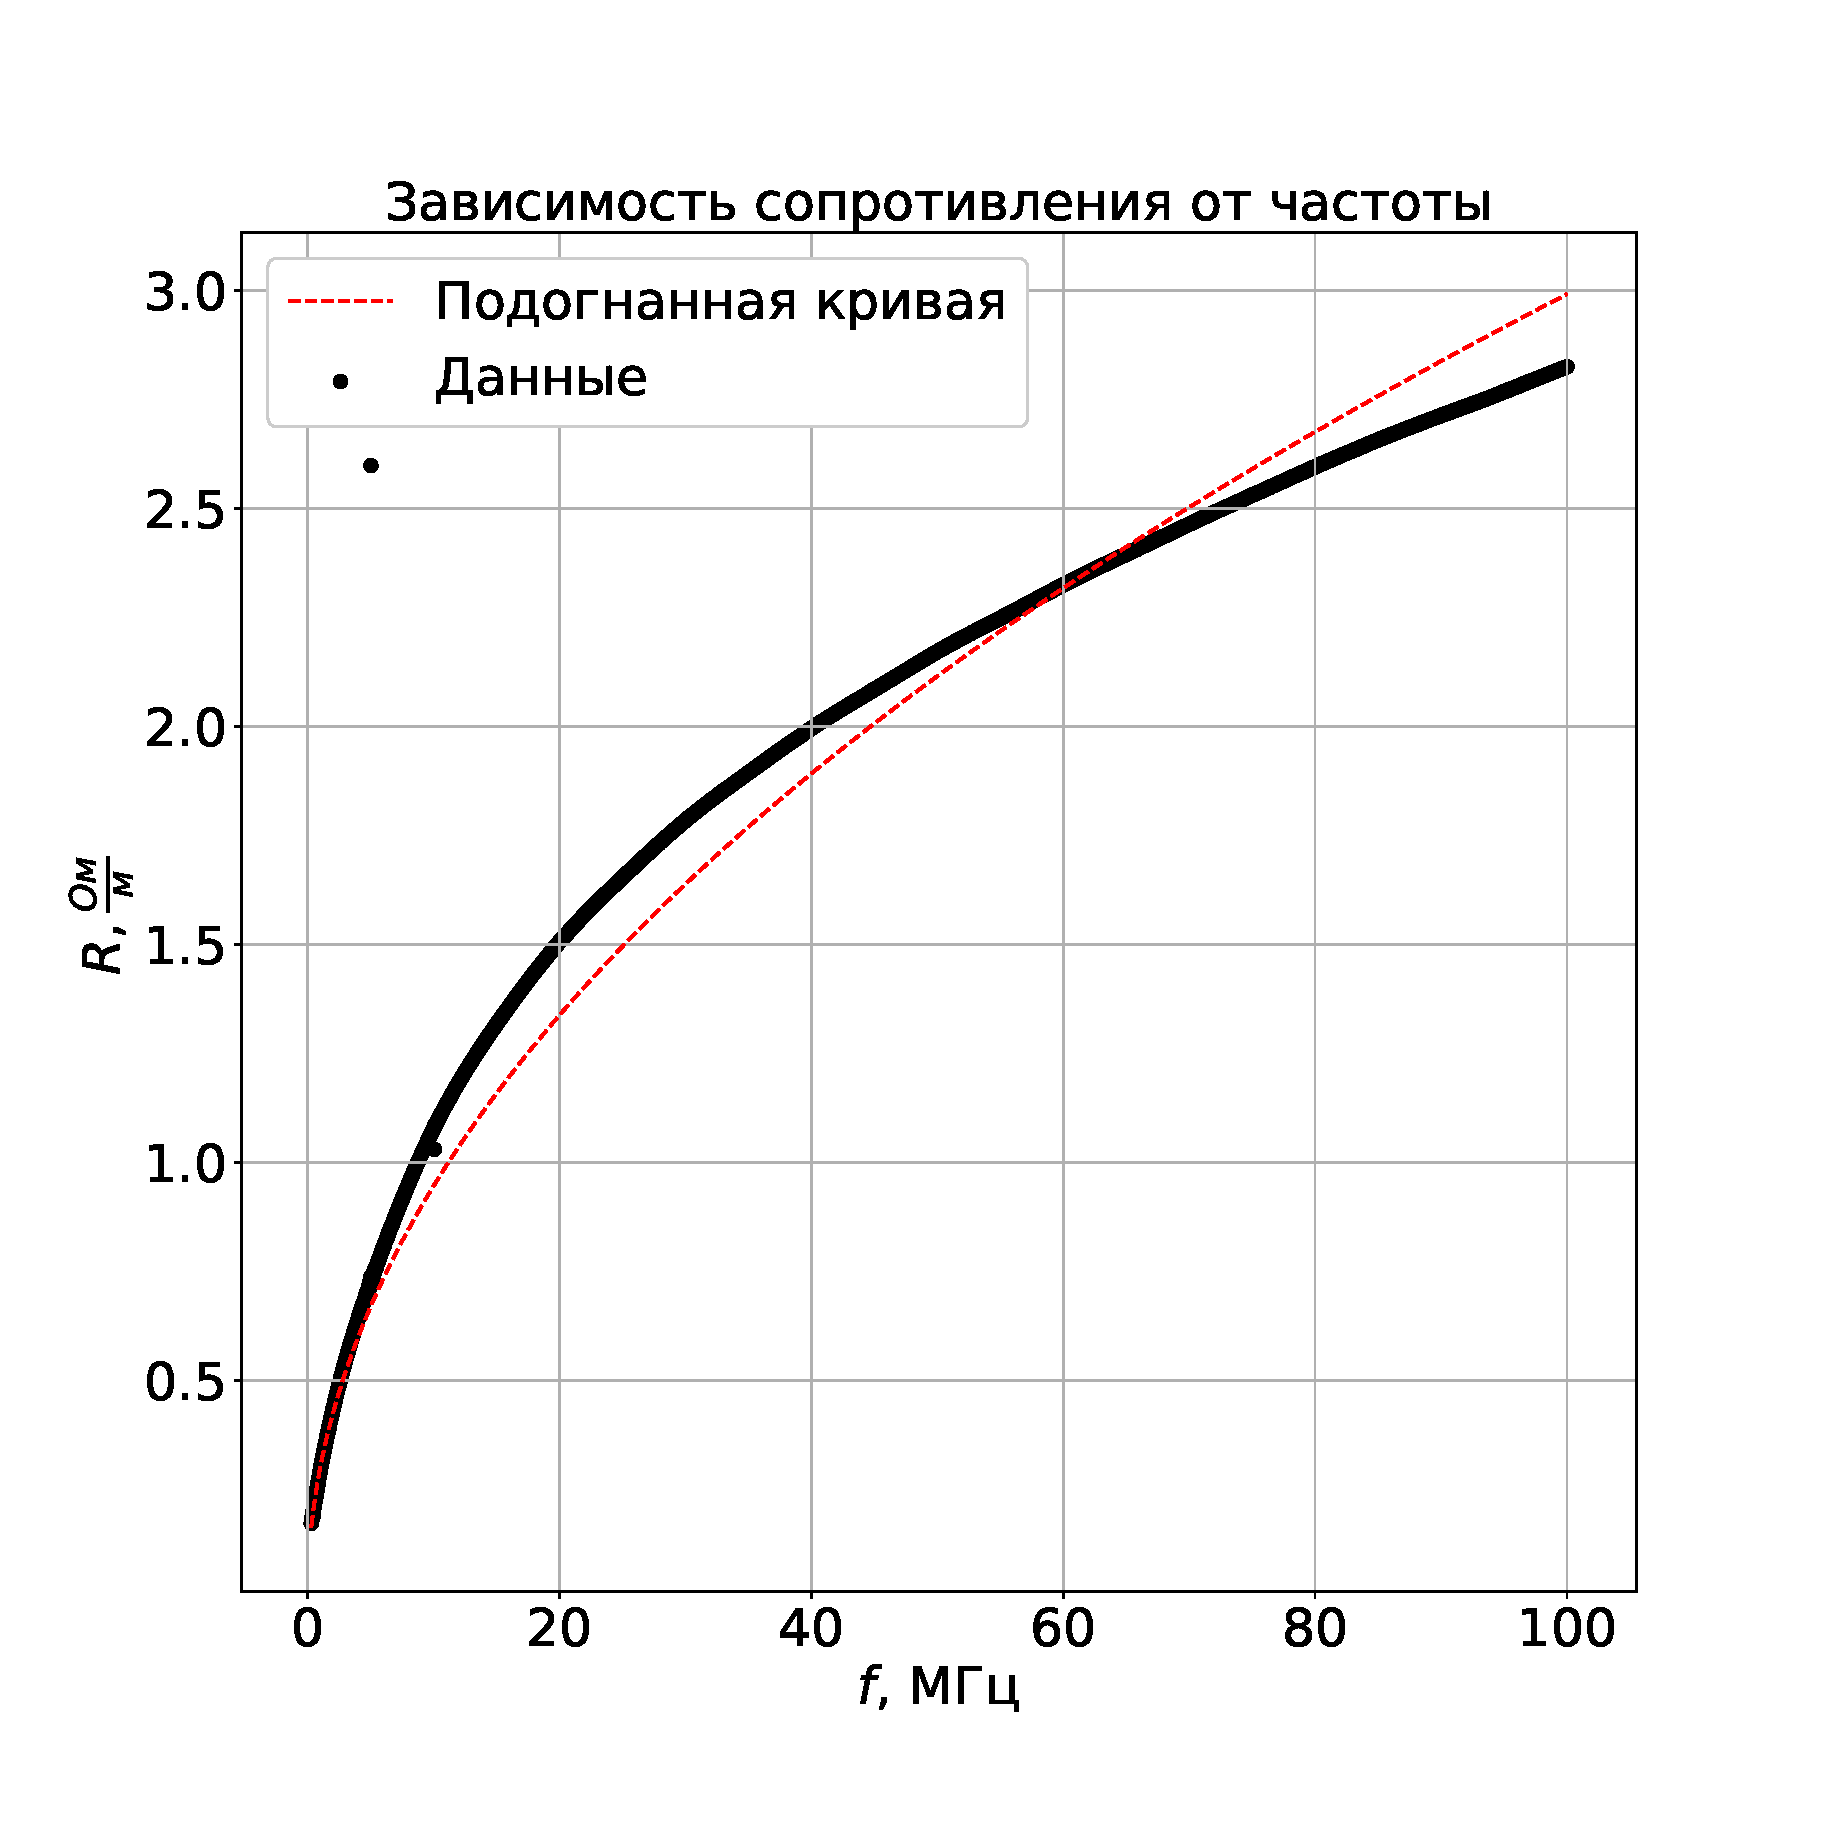
\includegraphics[width=.75\linewidth]{Lab3_4.eps}
			\caption{Зависимость сопротивления от частоты}
			\label{fig6}
		\end{figure}
		Кривая, согласно теории, подгонялась зависимостью $R = a_R \cdot \sqrt{f}$.
		\newpage
		\begin{figure}[h!]
			\centering
			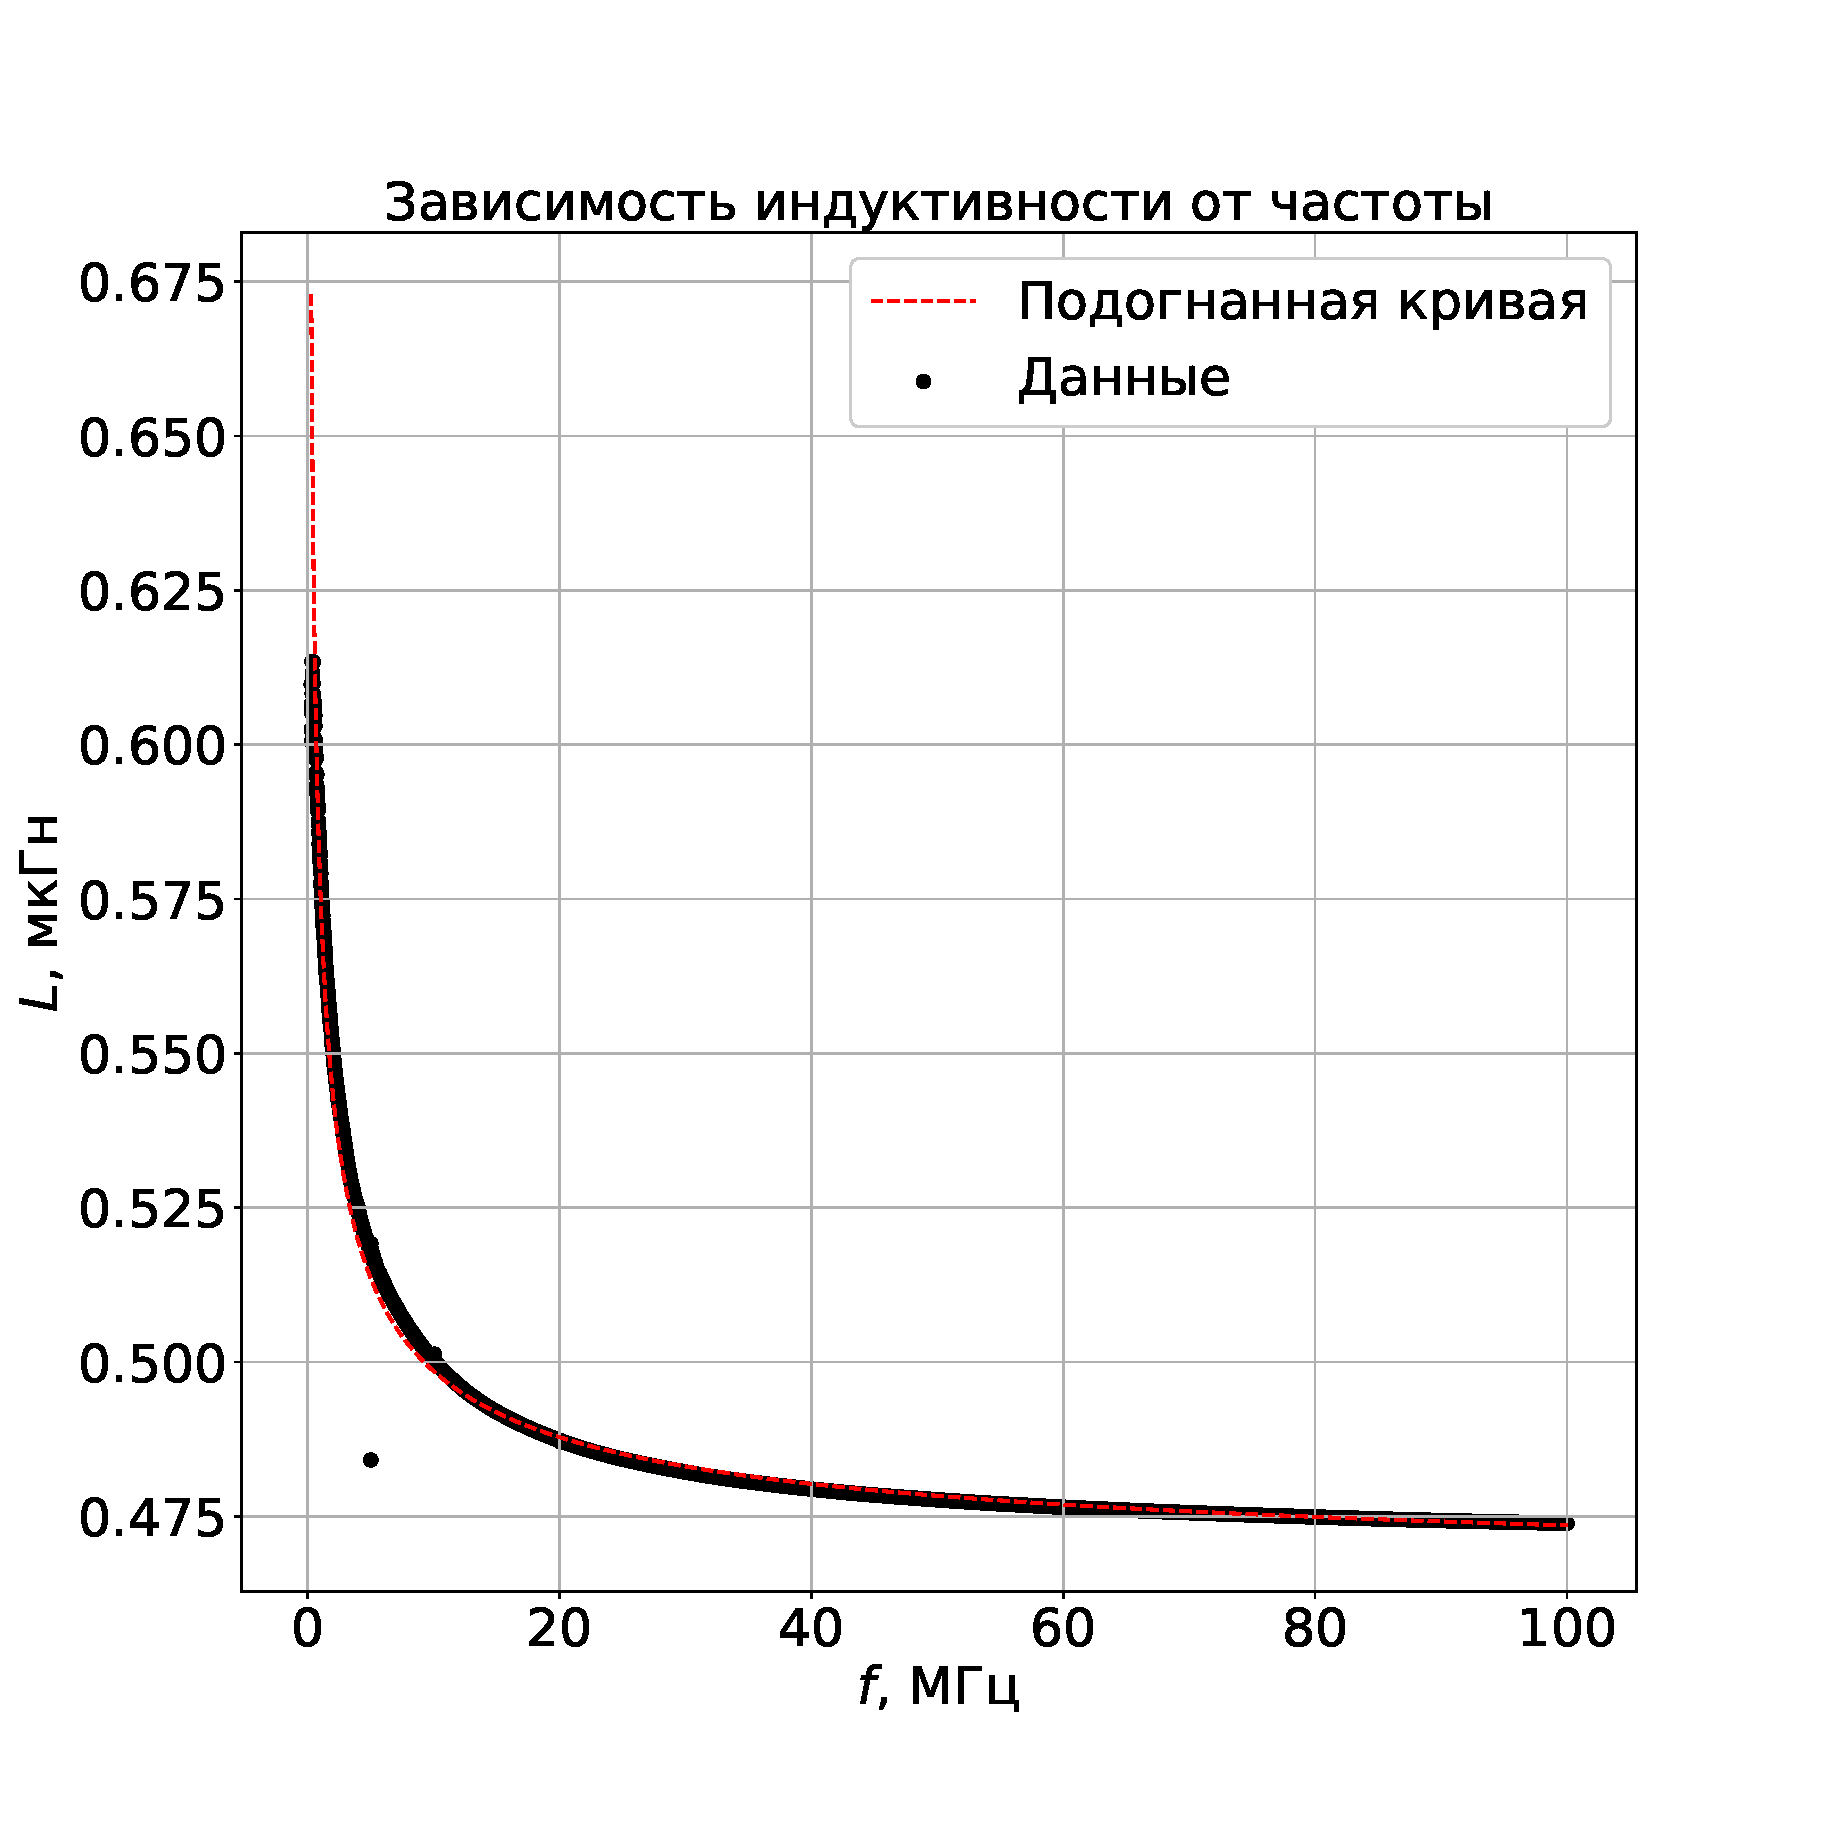
\includegraphics[width=.75\linewidth]{Lab3_5.eps}
			\caption{Зависимость индуктивности от частоты}
			\label{fig7}
		\end{figure}
		Кривая, согласно теории, подгонялась зависимостью $L = a_L \cdot \sqrt{\frac{1}{f}} +  b_L$.
		Получившиеся коэффициенты:
		\begin{equation}
			\begin{gathered}
				a_R = 0.29 \; \frac{\text{Ом}}{\text{м}} \cdot \text{МГц}^{-1/2}\\
				a_L = 0.11 \; \frac{\text{мкГн}}{\text{м}} \cdot \text{МГц}^{1/2}\\
				b_L = L_\infty =  0.46 \; \frac{\text{мкГн}}{\text{м}}
			\end{gathered}
		\end{equation}
		Теоретические коэффициенты (удельное сопротивление проводника взято из эксперимента со входным импедансом):
		\begin{equation}
			\begin{gathered}
				a_{Rt} = 0.33 \; \frac{\text{Ом}}{\text{м}} \cdot \text{МГц}^{-1/2}\\
				a_{Lt} = 0.10 \; \frac{\text{мкГн}}{\text{м}} \cdot \text{МГц}^{1/2}\\
				b_{Lt} = L_{\infty t} =  0.40 \; \frac{\text{мкГн}}{\text{м}}
			\end{gathered}
		\end{equation}
		Также из графика получаем удельное сопротивление материала проводника (среднее значение для всех точек на графике):
		\begin{equation}
			\rho \approx 2.9 \cdot 10^{-8} \text{Ом} \cdot \text{м}
		\end{equation}
		\section{Выводы}
		В ходе работы были получены различные параметры коаксиального кабеля. Геометрические размеры, удельные емкость, сопротивление и индуктивность, кроме того было получено удельное сопротивление материала проводника. Полученные экспериментальным путем удельное сопротивление и коэффициенты зависимостей индуктивности от частоты оказались достаточно близкими к теоретическим. Подогнанные кривые по теоретической зависимости хорошо легли на графики этих параметров. Это позволяет сказать, что теоретические предположения о малости потерь и пренебрежения различными эффектами были корректными в рамках исследования параметров такого кабеля.
\end{document}